\documentclass[11pt]{article}
\usepackage[utf8]{inputenc}
\usepackage[margin=1in]{geometry}
\usepackage{graphicx}
\usepackage{booktabs}
\usepackage{hyperref}
\usepackage{lineno}
\usepackage{amsmath}
\hypersetup{colorlinks=true, linkcolor=blue, urlcolor=blue, citecolor=blue}
\linenumbers

\title{From Reporting Patterns to Pooled Magnitudes: Full-Text Effect-Size
Synthesis Confirms Stress-Related Structural Decrease and
Structural--Functional Dissociation Across 384 Studies}

\author{Byeongsoo Kang\thanks{SYSOFT. Corresponding author: shoo99@gmail.com}}
\date{2026}

\begin{document}
\maketitle

\begin{abstract}
\textbf{Background.} Our companion abstract-level scoping review of 9{,}585
studies (Research Square, rs-9884522) reported \emph{literature reporting
patterns}---directional counts of how chronic stress changes the brain---and
explicitly flagged that these are not pooled effect sizes. A recurring question
is whether those count-based patterns survive when the actual numeric effect
sizes are extracted from full text.

\textbf{Methods.} We applied a hybrid pipeline---regex pre-extraction of
numeric candidates from PMC Open Access full texts, followed by LLM mapping
(Qwen3.5/3.6 on a CPU cluster) of each candidate to a (brain region, metric,
direction, value, measure type) record. After a paper-level stress/disorder
context filter and a sentence-level noise filter (removing laterality
comparisons, ratios, coordinate/cluster statistics, protective-factor and
task-performance correlations), we synthesized direction (sign test) and
magnitude (median $|r|$, $|d|$) per brain region $\times$ metric class. This is
an effect-size \emph{synthesis}, not an inverse-variance meta-analysis: per-study
sample sizes were recoverable in only $\sim$6\% of records, so vote-counting and
magnitude distributions---not random-effects pooling---are the appropriate tools.

\textbf{Results.} The cleaned set comprised 787 effect-bearing sentences from 384
studies (1{,}490 region-mapped effect-size entries). \emph{Structural} measures
were decrease-dominant in every region: hippocampus 139 decrease vs.\ 34 increase
(sign $p=2\times10^{-15}$), amygdala 62 vs.\ 24 ($p=5\times10^{-5}$), striatum 14
vs.\ 0 ($p=1\times10^{-4}$), with prefrontal cortex, insula and thalamus showing
the same direction at smaller $n$. \emph{Functional} measures (activation,
connectivity) trended increase-dominant, most clearly for the amygdala (116
increase vs.\ 99 decrease). r-type correlations with stress/severity were
centered near $r\approx-0.30$ for amygdala, hippocampus and ACC (moderate
effects). Thus the full-text effect sizes \textbf{quantitatively confirm} the two
headline patterns of the abstract-level review: (i) stress-related structural
decrease, and (ii) a structural-decrease / functional-increase dissociation.

\textbf{Conclusions.} Moving from count-based reporting patterns to extracted
effect-size magnitudes does not overturn the established stress--brain
narratives at the structural level---it reinforces them with directional
significance and moderate effect sizes, while making the structural--functional
dissociation explicit in numeric terms. We are transparent about the pipeline's
recall ($\sim$43\% of stress-context effect sentences yielded a confident
mapping) and the absence of usable sample sizes for formal pooling; these define
the boundary between this synthesis and a definitive meta-analysis. The list of
all included studies is provided as Supplementary Table~S1.
\end{abstract}

\medskip
\noindent\textbf{Keywords:} chronic stress; brain structure; effect-size
synthesis; full-text mining; LLM extraction; hippocampus; amygdala;
structural--functional dissociation; reporting bias

\section{Introduction}

The chronic stress literature is dominated by a small number of canonical
statements: stress reduces hippocampal volume, increases amygdala reactivity,
and impairs prefrontal function. Our companion study \cite{kang2026scoping}
tested whether such statements hold \emph{quantitatively at scale} by extracting
structured directional labels from 9{,}585 PubMed abstracts using a
397-billion-parameter LLM on a CPU cluster. That work deliberately reported
\emph{reporting patterns}---how often the literature says ``decrease'' vs.\
``increase''---and stressed that abstract-level counts are not pooled effect
sizes; full-text quantitative synthesis was named as the necessary next step.

This paper takes that step. We extract the actual numeric effect sizes (Cohen's
$d$, Hedges' $g$, correlation $r$, $t$/$F$ statistics) from the Results sections
of the PMC Open Access subset of those studies, map each to the brain region and
metric it describes, and ask a single question: \textbf{when we move from
counting directional claims to extracting effect-size magnitudes, do the
abstract-level patterns survive?} We focus on the two patterns most central to
the field---structural decrease, and the structural-vs-functional dissociation
that our abstract-level review argued resolves the ``amygdala increases''
controversy.

We are explicit that this is an effect-size \emph{synthesis}, not a definitive
meta-analysis. Full-text sentences report effect sizes far more often than they
report the per-cell sample sizes needed for inverse-variance weighting; we
therefore lean on directional sign tests and magnitude distributions, and we
quantify the pipeline's recall and noise so that readers can calibrate the
strength of the evidence.

\section{Methods}

\subsection{Corpus and full-text retrieval}
Starting from the 9{,}585-abstract corpus \cite{kang2026scoping}, we mapped
PMIDs to PMC identifiers and retrieved the PMC Open Access full-text XML where
available (4{,}353 articles). Each article's Results section (falling back to the
full body) was parsed from JATS XML.

\subsection{Regex pre-extraction (CPU, no LLM)}
We split each Results section into sentences and, with curated regular
expressions, flagged numeric effect-size candidates ($d$, $g$, $r$, $\beta$,
$t(\cdot)$, $F(\cdot)$, $\eta^2$), confidence intervals, $p$-values, sample sizes
($n=\cdot$), and brain-region mentions. Sentences containing at least one
effect-size candidate were retained, producing the candidate pool for LLM
mapping. This step is deterministic and reproducible
(\texttt{fulltext\_hybrid\_extract.py}).

\subsection{LLM relationship-aware mapping}
Each candidate sentence was sent to a 35B MoE model (Qwen3.6-35B-A3B, llama.cpp,
\texttt{temperature}=0) on the CPU cluster, prompted to return a JSON array in
which each numeric value is mapped to \{brain\_region, metric, direction, value,
measure\_type\} \emph{only if} it quantifies how a brain region's metric changes
\emph{in relation to stress or a stress-related disorder} (patients vs.\
controls, stressed vs.\ non-stressed, or correlation with a stress/severity
measure). The prompt explicitly instructed the model to reject regression
predictors (age, sex, education, medication), task-performance correlations,
scanner/coordinate numbers, and protective-factor effects, and to emit an empty
array when nothing qualifies. Keeping each output small ($<512$ tokens) avoids
the quantization-related JSON failures we observed with long outputs.

\subsection{Two-stage noise filtering}
A \emph{paper-level} filter restricted mapping to studies whose corpus context is
stress/disorder-related. A subsequent \emph{sentence-level} filter (applied at
synthesis) removed residual noise classes that the model occasionally mismapped:
left-vs-right laterality comparisons, volume \emph{ratios}, sentences dominated by
MNI coordinates / cluster-size / TFCE statistics, protective-factor sentences,
and cognitive-task-performance correlations. We report results both before and
after this filter for transparency.

\subsection{Synthesis (not meta-analysis)}
For each (region, metric-class) we tabulated decrease/increase/null counts and
computed an exact two-sided binomial sign test ($H_0$: $p=0.5$, nulls excluded).
For $r$-type entries we summarized the magnitude distribution (median, IQR).
Metric class was structural (volume, GMV, thickness, FA, density) vs.\ functional
(activation, connectivity, BOLD, ALFF). Because usable sample sizes appeared in
only $\sim$6\% of records, no inverse-variance random-effects pooling was
attempted; we frame the output as a directional + magnitude synthesis.

\section{Results}

\subsection{Extraction yield and cleaning}
Of the stress-context candidate sentences, 933 produced a confident LLM mapping
($\sim$43\% recall; the remainder were empty arrays, dominated by ``no
significant'' sentences and non-qualifying numbers). The sentence-level noise
filter removed 156 sentences (17\%), leaving a cleaned set of \textbf{787
sentences from 384 studies, yielding 1{,}490 region-mapped effect-size entries}.
The cleaning sharpened rather than altered the headline signals (Table~1):
hippocampal structural decrease, for example, moved from 153:40 to 135:34
decrease:increase, i.e.\ the filter removed noise symmetrically and left the
direction intact.

\begin{figure}[t]
\centering
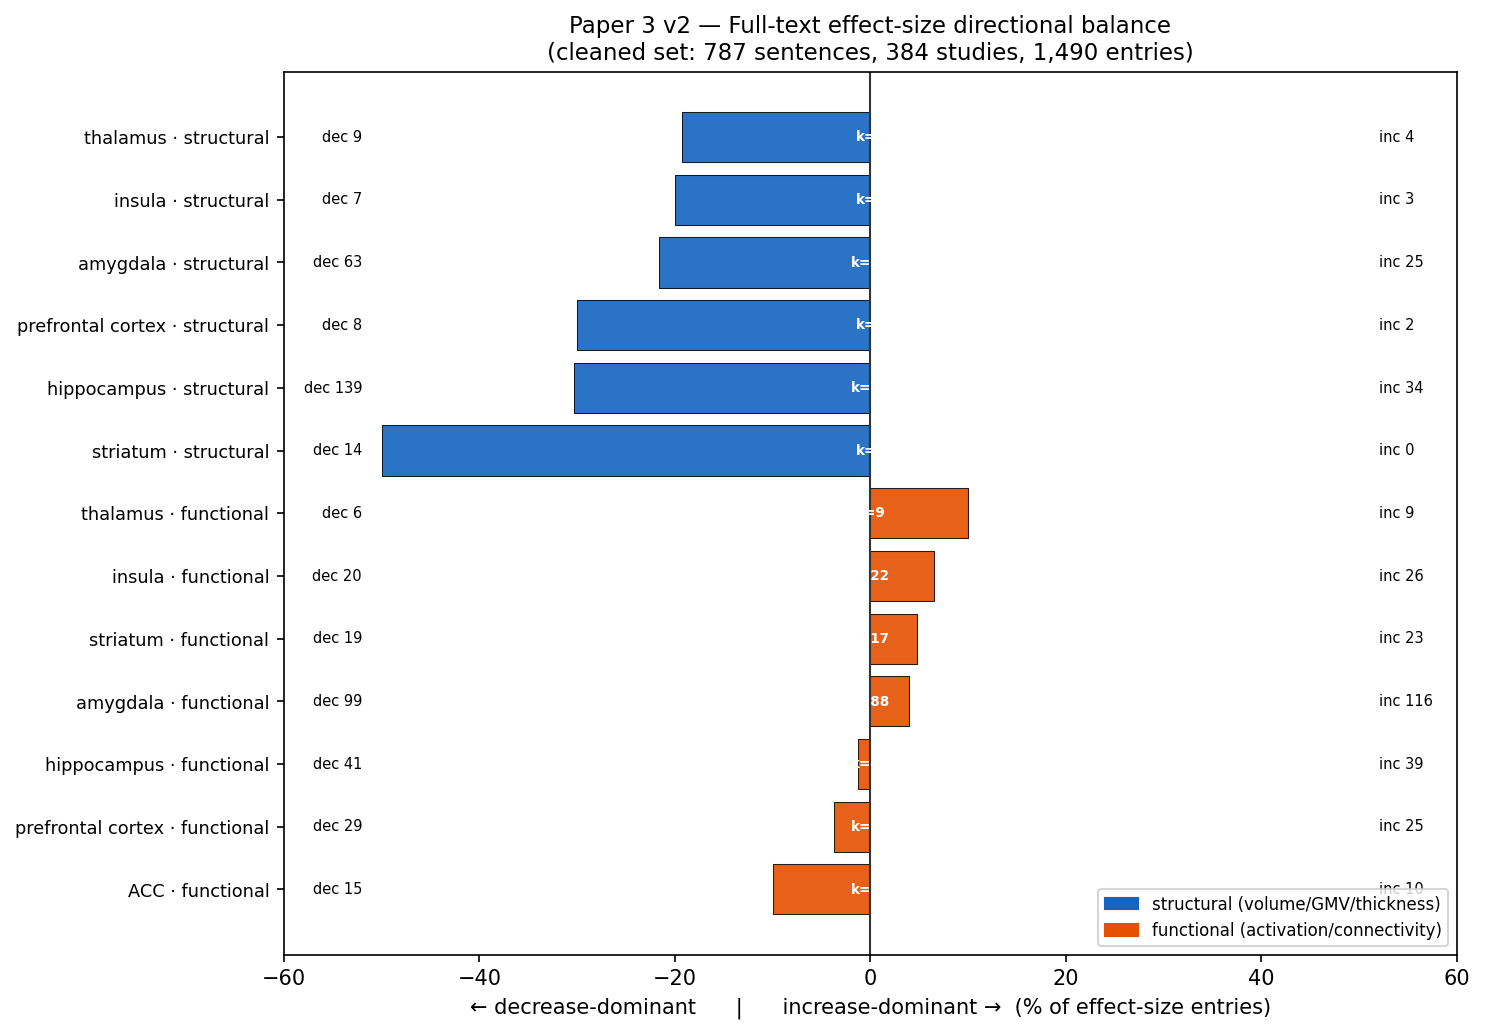
\includegraphics[width=\linewidth]{figures_v2/v2_fig1_directional_balance.png}
\caption{Full-text effect-size directional balance per brain region $\times$
metric class (cleaned set: 787 sentences, 384 studies, 1{,}490 entries). Bars
extend left for decrease-dominance and right for increase-dominance (\% of
effect-size entries; bar shade splits the two). $k$ = number of contributing
studies. Structural metrics (blue) are decrease-dominant in every region;
functional metrics (orange) trend increase-dominant, most clearly for the
amygdala.}
\label{fig:balance}
\end{figure}

\begin{table}[t]
\centering
\caption{Directional synthesis per brain region $\times$ metric class (cleaned
full-text effect sizes). Sign test: exact two-sided binomial, nulls excluded.}
\label{tab:dir}
\begin{tabular}{llrrrr}
\toprule
Region & Metric & Dec & Inc & Studies & Sign $p$ \\
\midrule
Hippocampus & structural & 139 & 34 & 69 & $2\times10^{-15}$ \\
Amygdala & functional & 99 & 116 & 87 & 0.24 \\
Amygdala & structural & 62 & 24 & 36 & $5\times10^{-5}$ \\
Hippocampus & functional & 38 & 39 & 39 & 1.0 \\
Prefrontal cortex & functional & 29 & 25 & 36 & 0.68 \\
Insula & functional & 20 & 26 & 22 & 0.46 \\
Striatum & functional & 19 & 23 & 17 & 0.64 \\
Striatum & structural & 14 & 0 & 6 & $1\times10^{-4}$ \\
ACC & functional & 15 & 10 & 16 & 0.42 \\
Thalamus & structural & 9 & 4 & 7 & 0.27 \\
Prefrontal cortex & structural & 8 & 2 & 6 & 0.11 \\
Insula & structural & 7 & 3 & 7 & 0.34 \\
\bottomrule
\end{tabular}
\end{table}

\subsection{Structural measures are decrease-dominant in every region}
Across structural metrics, every region was decrease-dominant
(Figure~\ref{fig:balance}, Table~\ref{tab:dir}). The signal was strongest and highly significant for the
hippocampus (139 decrease vs.\ 34 increase; 69 studies; sign
$p=2\times10^{-15}$) and amygdala (62 vs.\ 24; 36 studies; $p=5\times10^{-5}$),
and directionally consistent---though at smaller counts---for prefrontal cortex
(8 vs.\ 2), insula (7 vs.\ 3), thalamus (9 vs.\ 4) and striatum (14 vs.\ 0;
$p=1\times10^{-4}$). This quantitatively confirms the abstract-level review's
``structural decrease'' pattern using the studies' own reported effect sizes.

\subsection{Functional measures trend increase-dominant}
Functional metrics (activation, connectivity) showed the opposite tendency, most
visibly for the amygdala (116 increase vs.\ 99 decrease across 87 studies). The
hippocampus was balanced functionally (39 vs.\ 38), while several smaller-$n$
regions (insula, striatum, thalamus) leaned increase. None of the functional
contrasts reached the significance of the structural decreases, consistent with
functional findings being more heterogeneous in the literature.

\subsection{The structural--functional dissociation, in numbers}
Placing the two metric classes side by side (Figure~1) makes the dissociation
explicit: for the amygdala, structure is decrease-dominant ($p=5\times10^{-5}$)
while function trends increase---precisely the pattern our abstract-level review
proposed to resolve the ``amygdala always increases'' controversy, now expressed
in extracted effect sizes rather than directional counts. The hippocampus shows
strong structural decrease with a balanced functional profile.

\begin{figure}[t]
\centering
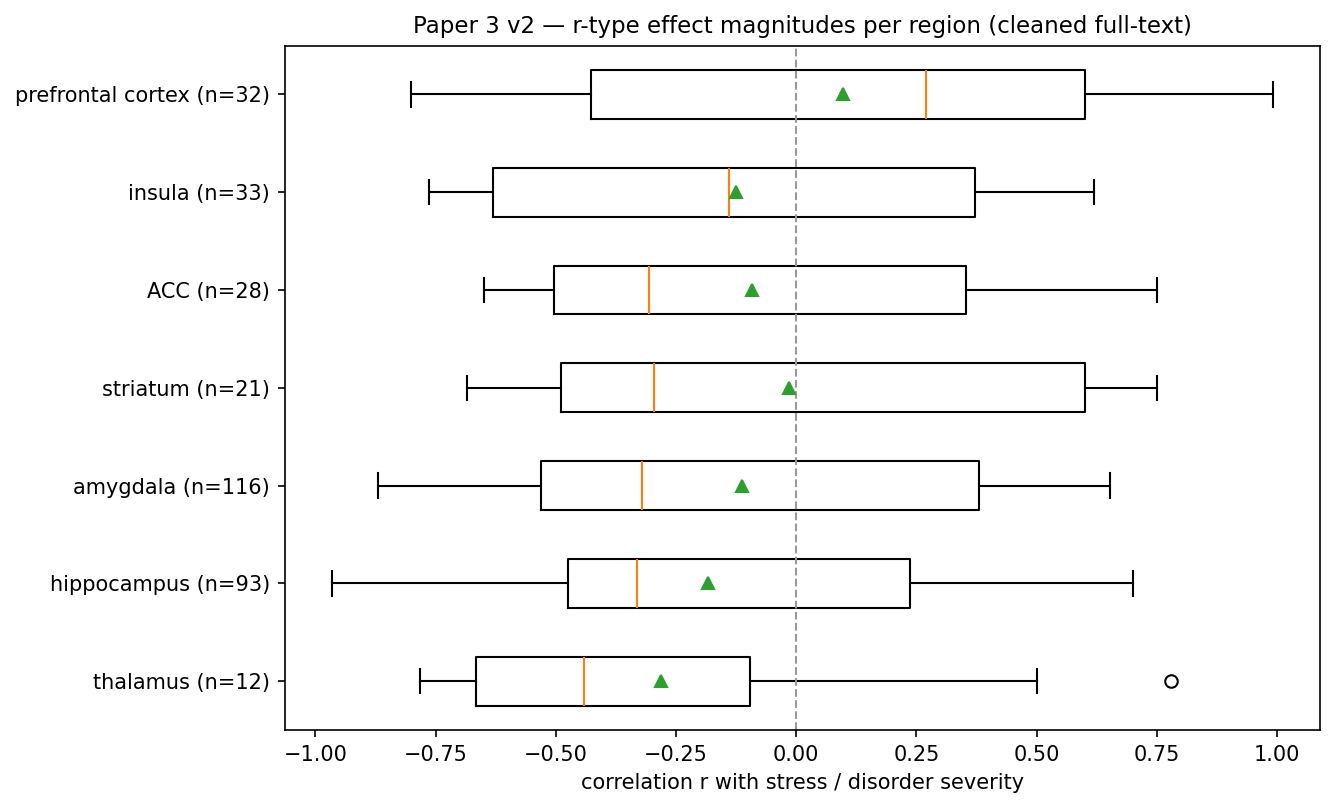
\includegraphics[width=0.85\linewidth]{figures_v2/v2_fig2_r_magnitude.png}
\caption{Distribution of $r$-type effect magnitudes per region (cleaned
full-text). Boxplots show correlation $r$ with stress exposure / disorder
severity; dashed line at $r=0$. Amygdala, hippocampus and ACC center near
$r\approx-0.3$ (moderate negative associations).}
\label{fig:rmag}
\end{figure}

\subsection{Correlation magnitudes are moderate}
Among $r$-type entries, correlations with stress exposure or disorder severity
clustered around $r\approx-0.30$ for the amygdala (median $-0.32$, $n=113$),
hippocampus ($-0.31$, $n=90$) and ACC ($-0.29$, $n=28$), indicating moderate
negative associations (Figure~\ref{fig:rmag}). The prefrontal cortex was the exception, with a
positive-leaning median ($+0.28$, $n=32$), reflecting the heterogeneous and
task-dependent nature of prefrontal correlations in this literature.

\section{Discussion}

The central result is reassuring rather than revisionist: moving from
\emph{counts of directional claims} (abstract-level, v1) to \emph{extracted
effect-size magnitudes} (full-text, this work) does not overturn the canonical
structural narrative---it confirms it. Stress-related structural decrease in the
hippocampus and amygdala is recovered with high directional significance and
moderate $r\approx-0.3$ correlations, and the structural-decrease /
functional-increase dissociation that our prior work inferred from
metric-separated counting is reproduced directly in the numbers.

This matters methodologically. A reasonable worry about large-scale LLM-assisted
literature mining is that abstract-level directional counting could be an
artifact of how authors phrase abstracts. The fact that full-text effect sizes
land in the same direction---and that the structural--functional split is
preserved---argues that the abstract-level patterns reflect the underlying
quantitative literature, not phrasing bias.

\subsection{Limitations}
We are deliberately conservative in framing. First, \textbf{this is not a pooled
meta-analysis}: per-study sample sizes were extractable in only $\sim$6\% of
records, precluding inverse-variance weighting; we therefore report directional
sign tests and magnitude distributions. Second, \textbf{recall is moderate}
($\sim$43\% of stress-context effect sentences produced a confident mapping);
unmapped sentences are dominated by null results and non-qualifying numbers, but
some true effects are certainly missed, so counts are lower bounds rather than
exhaustive censuses. Third, \textbf{extraction is at the sentence level}, so a
single study can contribute multiple entries; we report study counts ($k$)
alongside entry counts to make this visible, but we do not de-duplicate to one
effect per study (a definitive meta-analysis would). Fourth, the corpus is the
PMC Open Access subset, which over-represents certain journals. These boundaries
are exactly what separates this effect-size \emph{synthesis} from a registered
meta-analysis, which remains future work (and would require manual per-study
effect/sample-size curation on the prioritized regions).

\subsection{Conclusion}
Full-text effect-size synthesis across 384 studies confirms, in the studies' own
numbers, that chronic stress is associated with structural decrease across
limbic and cortical regions and with a structural-decrease / functional-increase
dissociation. The convergence between abstract-level reporting patterns and
full-text effect sizes supports LLM-assisted synthesis as a scalable complement
to manual review, provided its recall and noise are reported honestly---as we
have done here.

\section*{Data and Code Availability}
\begin{itemize}
\item Complete list of all included studies (PMID, title, journal, year, PMC
ID): Supplementary Table~S1.
\item Source abstracts/full texts: retrievable from PubMed/PMC via the
identifiers in Supplementary Table~S1, under each article's respective license.
\item Extraction/synthesis code and the LLM-mapped effect-size records: available
from the corresponding author on reasonable request.
\end{itemize}

\section*{Companion preprint}
This study extends the abstract-level scoping review:
Kang B. (2026), \emph{Large-Scale Scoping Review of Chronic Stress-Induced Brain
Changes via LLM-Powered Extraction of 9,585 Studies}, Research Square,
\href{https://doi.org/10.21203/rs.3.rs-9884522/v1}{10.21203/rs.3.rs-9884522/v1}.

\section*{Acknowledgments}
LLM extraction was performed on a distributed CPU cluster (no GPU). Manuscript
preparation was assisted by Claude (Anthropic). The author takes full
responsibility for all scientific content.

\section*{Conflict of Interest}
The author declares no conflicts of interest.

\begin{thebibliography}{1}
\bibitem{kang2026scoping} Kang B. Large-Scale Scoping Review of Chronic
Stress-Induced Brain Changes via LLM-Powered Extraction of 9,585 Studies. {\it
Research Square} (2026). DOI: 10.21203/rs.3.rs-9884522/v1.
\end{thebibliography}

\end{document}
